\documentclass[12pt]{beamer}
\usetheme{Warsaw}
\usepackage{times}
\usepackage[T1]{fontenc}
\usepackage[utf8]{inputenc}
\usepackage{graphicx}
\usepackage{tikz}
\usepackage{listings}

%\usepackage{pgfpages}
%\pgfpagesuselayout{4 on 1}[a4paper,border shrink=5mm]

\title{Introducción a Matlab y Octave}
%\subtitle{Lesson 0}
\author{Guillem Borrell\\
Lab. de Mecánica de Fluidos Computacional}

\begin{document}

\lstset{language=Matlab,
  backgroundcolor=\color{black!10},
  numbers=left,
  basicstyle=\small\ttfamily,
  keywordstyle=\color{blue},
  extendedchars=true,
  inputencoding=utf8,
  showspaces=false}

\begin{frame}
  \titlepage
\end{frame}

\begin{frame}
  \frametitle{Antes de empezar}
  \begin{itemize}
  \item Guillem Borrell i Nogueras.
    \begin{itemize}
    \item Ingeniero Aeronáutico.
    \item DNS Flujos turbulentos.
    \item Supercomputación.
    \end{itemize}
  \item  \url{http://iimyo.forja.rediris.es/}
    \begin{itemize}
      \item Introducción Informal a Matlab y Octave.
      \item Matemáticas en Ingeniería con Matlab y Octave.
      \item Transparencias y ejercicios de este curso.
      \item Material de otros cursos.
    \end{itemize}
  \end{itemize}
\end{frame}


\begin{frame}
\frametitle{Recordad...}
\begin{itemize}
\item Ningún lenguaje se aprende por osmosis \pause
\item Cuando uno se hace mayor cada vez tiene menos paciencia \pause
\end{itemize}


\end{frame}


\begin{frame}
  \tableofcontents[pausesections]
\end{frame}

\section{Introducción}

\begin{frame}
  \frametitle{Objetivos}
  \begin{itemize}
  \item Introducción a la programación.
  \item Aprender un poquito de Matlab
  \item Facilitar vuestro aprendzaje.
  \item Ahorraros futuros disgustos.
  \end{itemize}
\end{frame}

\begin{frame}
  \begin{Huge}
    \begin{center}
      Matlab no es una herramienta de cálculo simbólico.
    \end{center}
  \end{Huge}
  \pause
  Matlab es un lenguaje de programación
\end{frame}

\begin{frame}
  \frametitle{Matlab es un lenguaje de programación}
  \begin{itemize}
  \item Orientado a Cálculo Numérico
  \item Nada de Cálculo Simbólico
    \begin{itemize}
    \item Imaginadlo como una gran calculadora
    \end{itemize}
  \item Si es un lengaje de programación
    \begin{itemize}
    \item No es una hoja de cálculo
    \item No es un juguete
    \item No es la solución a todos nuestros problemas.
    \end{itemize}
  \end{itemize}
\end{frame}

\begin{frame}
  \frametitle{¿Qué es Matlab?}
  \begin{itemize}
    \item{Un lenguaje de programación}
    \item{Un lenguaje de programación \emph{interpretado}}
    \item{Un lenguaje de programación \emph{interactivo}}
  \end{itemize}
  \begin{center}
    \textbf{Usar Matlab == Programar en Matlab}
  \end{center}
\end{frame}


\defverbatim[colored]\testcode{
\begin{lstlisting}
f = @(x) quad(@(y) exp(-y.^2),0,y)
\end{lstlisting}
}
\begin{frame}
  \frametitle{¿Cómo de potente?}
Esto es Matlab avanzado

\[ f(x) = \int_0^x \exp(-y^2) dy \]

\testcode

Por cierto, esto es Cálculo Numérico
\end{frame}

\begin{frame}
  \frametitle{¿Por qué Matlab?}

  \begin{itemize}
  \item Herramienta más extendida en Ciencia e Ingeniería
  \item Estándar de facto para escribir pequeños programas.
  \item Enorme librería estándar
  \item Toolboxes para casi cualquier disciplina de la Ingeniería
  \end{itemize}

\end{frame}

\section{Fundamentos de Programación}

\defverbatim[colored]\testcode{
\begin{lstlisting}
a = 1;
\end{lstlisting}
}
\begin{frame}
  \frametitle{Variables y literales}
\testcode
\begin{itemize}
\item \texttt{a} es una variable
\item \texttt{=} es el operador asignación
\item \texttt{1} es el literal que significa el número 1
\end{itemize}
\begin{center}
  ¿Qué significa todo esto?
\end{center}
\end{frame}

\begin{frame}
  \frametitle{El significado de todo esto}
  \begin{itemize}
  \item Las variables almacenan en memoria
  \item El operador asignación asigna cualquier cosa a una variable
  \item Todos los cálculos van a la derecha del operador
  \item Los cálculos son cualquier operación entre variables y literales
  \end{itemize}
\end{frame}

\begin{frame}
  \frametitle{Variables}
  \begin{itemize}
  \item Cualquier palabra puede convertirse en variable
  \item Siempre que no use un caracter reservado como \texttt{+},
    \texttt{-}, \texttt{*}, \texttt{/}, \texttt{\^}, \texttt{.}, ...
  \item O no sea un nombre reservado como \texttt{ans} or \texttt{pi}
  \item Una variable puede almacenar cualquier valor.
  \end{itemize}
\end{frame}

\begin{frame}
  \frametitle{Literales}
  \begin{itemize}
  \item Es la manera que tenemos de introducir un valor.
  \item Hay un literal para prácticamente cualquier valor en Matlab:
    escalares, vectores, funciones...
  \item Prácticamente significa que no están todos, pero los que
    faltan no los echaremos de menos.
  \end{itemize}
\pause
Pero antes de programar, algo de evangelismo.
\end{frame}

\subsection{El entorno de desarrollo Matlab}
\begin{frame}
  \frametitle{Herramientas}
Partes del entorno de escritorio Matlab
\begin{itemize}
\item La consola
\item El editor
\item El explorador
\item El debugger
\end{itemize}
Aprenderemos sólo a utilizar la consola y el editor
\end{frame}

\begin{frame}
  \frametitle{La consola}

\pgfimage[width=\linewidth]{../_static/principal_col}

\end{frame}

\begin{frame}
  \frametitle{El editor}
\pgfimage[width=\linewidth]{../_static/editor}
\end{frame}

\begin{frame}
\frametitle{Scripts}
\begin{itemize}
\item Un script es un programa
\item Un programa es una secuencia de instrucciones ejecutables
\item Un programa no depende de variables externas
\item Se guarda en un archivo \emph{.m} en el \emph{directorio
  de trabajo}
\item Se ejecuta escribiendo el nombre del archivo en la consola o
  pulsando \texttt{F5} en el editor.
\end{itemize}
\end{frame}


\defverbatim[colored]\testcode{
\begin{lstlisting}
aprsin = @(x) x - x.^3/6;
x = linspace(-pi,pi,100);
plot(x,aprsin(x),x,sin(x));
\end{lstlisting}
}

\begin{frame}
\frametitle{Nuestro primer script}
En un archivo nuevo del editor
\testcode
Lo guardamos con el nombre \texttt{comparar.m} \emph{en el directorio
  de trabajo}. Luego pulsamos \texttt{F5}
\end{frame}


\begin{frame}
\frametitle{El resultado}
  \begin{figure}[h]
    \centering{}
    \pgfimage[width=8cm]{../_static/aprsin.pdf}
  \end{figure}
\end{frame}

\subsection{El intérprete Octave}
\begin{frame}
  \frametitle{Octave}
  \begin{itemize}
  \item Octave es un intérprete libre y gratuito del lenguaje Matlab
  \item Proporciona el intérprete y la consola interactiva, nosotros
    debemos proporcionar el resto
  \item Proporciona aproximadamente el 90\% del lenguaje y el 30\% de
    los toolkits.
  \end{itemize}
\end{frame}

\section{El lenguaje de programación Matlab}
\subsection{Tipos y literales}

\defverbatim[colored]\testcode{
\begin{lstlisting}
a = 1.234;
\end{lstlisting}
}
\begin{frame}
  \frametitle{Escalar}
  \begin{itemize}
  \item Un escalar es un número.
    \pause
  \item Sí, sólo un número.
  \item Pero a partir del escalar generamos el resto de tipos
  \item La coma decimal es un punto.
  \end{itemize}
  \testcode
\end{frame}

\begin{frame}
  \frametitle{Operaciones escalares}
  \begin{itemize}
  \item Suma. \texttt{+}
  \item Resta, Número negativo. \texttt{-}
  \item Multiplicación. \texttt{.*}
  \item División. \texttt{./}
  \item Potencia. \texttt{.\^}
  \end{itemize}
\end{frame}

\begin{frame}
  \frametitle{funciones escalares}
  \begin{itemize}
  \item \texttt{exp},\texttt{log},\texttt{log10},\texttt{sqrt}...
  \item \texttt{sin},\texttt{cos},\texttt{tan}...
  \item \texttt{asin},\texttt{acos},\texttt{atan}...
  \item \texttt{sinh},\texttt{cosh}...
  \item \texttt{gamma},\texttt{beta},\texttt{erf},\texttt{sinc}...
  \end{itemize}
\end{frame}

\defverbatim[colored]\testcode{
\begin{lstlisting}
>> exp(1.0i * pi) - 1
\end{lstlisting}
}

\begin{frame}
  \frametitle{Operaciones aritméticas}
  \[ exp(i \pi) - 1 = 0  \]
  \testcode
\end{frame}

\begin{frame}
  \frametitle{Otros tipos}
  \begin{itemize}
  \item La unidad imaginaria es \emph{i}, \emph{j}, \emph{I} o \emph{J}
  \item Las cadenas de texto se introducen entre comillas simples
  \item Los tipos lógicos son \emph{true} y \emph{false}.  \emph{true}
    es $\not \equiv 0$ y \emph{false} es $\equiv 0$
  \end{itemize}
\end{frame}

\defverbatim[colored]\testcode{
\begin{lstlisting}
>> % Este comando sera ignorado
>> 'hola' % 'Hola,Matlab!'
ans = hola

>> 'hola';
>> 'hola', 'que tal'
ans = hola
ans = que tal

>> 'hola', ...
'que tal'
ans = hola
ans = que tal
\end{lstlisting}
}

\begin{frame}
\frametitle{Caracteres especiales}
\testcode
\end{frame}


\defverbatim[colored]\testcode{
\begin{lstlisting}
  >> a = pi
  a = 3.1416
  >> a(1)
  ans = 3.1416
  >> a(1,1)
  ans = 3.1416
  >> a(1,1,1)
  ans = 3.1416
\end{lstlisting}
}

\begin{frame}
  \frametitle{Mira qué curioso}
  \testcode
\end{frame}

\begin{frame}
\frametitle{Escribir matrices}
\begin{itemize}
  \item El espacio o la coma separan elementos de la misma fila
  \item El retorno de carro o el punto y coma separa filas
\end{itemize}
\[ \left(
\begin{array}{ccc}
1&2&3\\
4&5&6\\
7&8&9
\end{array} \right)
\]
\end{frame}


\defverbatim[colored]\testcode{
\begin{lstlisting}
M=[1,2,3;4,5,6;7,8,9];
\end{lstlisting}
}

\begin{frame}
\frametitle{Ejercicio 1}
\testcode
Escribir 
\[ \left(
\begin{array}{ccc}
1&2&3\\
4&5&6\\
7&8&9
\end{array} \right)
\]
de otros 3 modos posibles.
\end{frame}

\begin{frame}
\frametitle{Subíndices}
\begin{itemize}
  \item En Matlab el primer índice cuenta elementos en la columna
  \item El segundo índice cuenta elementos en la fila
  \item \emph{Pero} un vector es siempre fila a no ser que se diga lo
    contrario.
  \item El truco es que no nos preocupen las filas y las columnas,
    sólo los índices
\end{itemize}
\[ M_{ij} = M(i,j) \]
\end{frame}

\defverbatim[colored]\testcode{
\begin{lstlisting}
>> v(4)=2
v =

   0   0   0   2

>> w(4,1)=2
w =

   0
   0
   0
   2
\end{lstlisting}
}
\begin{frame}
\frametitle{No hay quien te entienda}
\testcode
\end{frame}

\defverbatim[colored]\testcode{
\begin{lstlisting}
>> v=[1,2,3,4,5];
>> v(4)
ans = 4
\end{lstlisting}
}

\begin{frame}
\frametitle{Un vector...}
\[v = (1,2,3,\textcolor{red}{4},5) \]
\testcode
\end{frame}

\defverbatim[colored]\testcode{
\begin{lstlisting}
>> M=[1,2,3;4,5,6;7,8,9];
>> M(2,3)
ans =  6
\end{lstlisting}
}

\begin{frame}
\frametitle{Una matriz...}
\[ \left(
\begin{array}{ccc}
1&2&3\\
4&5&\textcolor{red}{6}\\
7&8&9
\end{array} \right)
\]
\testcode
\end{frame}


\defverbatim[colored]\testcode{
\begin{lstlisting}
>> M([1,2],[2,3])
ans =

   2   3
   5   6
\end{lstlisting}
}

\begin{frame}
\frametitle{Podemos indexar con vectores}
\[ \left(
\begin{array}{ccc}
1&\textcolor{red}{2}&\textcolor{red}{3}\\
4&\textcolor{red}{5}&\textcolor{red}{6}\\
7&8&9
\end{array} \right)
\]
\testcode
\end{frame}

\defverbatim[colored]\testcode{
\begin{lstlisting}
>> M(2,:)
ans =

   4   5   6
\end{lstlisting}
}

\begin{frame}
\frametitle{O con índices mudos}
\[ \left(
\begin{array}{ccc}
1&2&3\\
\textcolor{red}{4}&\textcolor{red}{5}&\textcolor{red}{6}\\
7&8&9
\end{array} \right)
\]
\testcode
\end{frame}

\defverbatim[colored]\testcode{
\begin{lstlisting}
\end{lstlisting}
}

\defverbatim[colored]\testcode{
\begin{lstlisting}
>> 0:2:10
ans =
   0   2   4   6   8  10

>> 0:5
ans =
  0  1  2  3  4  5
\end{lstlisting}
}


\begin{frame}
\frametitle{Secuencias}
\begin{itemize}
\item Es una abreviatura común para escribir un vector fila
\item La sintaxis es \texttt{inicio:incremento:final}
\end{itemize}
\testcode
\end{frame}

\begin{frame}
\frametitle{Ejercicio 2} 
Crear la matriz siguiente y extraer de ella la submatriz marcada en rojo.
\[ \left( \begin{array}{ccccc}
11&12&13&14&15\\
21&22&23&24&25\\
31&32&\textcolor{red}{33}&\textcolor{red}{34}&\textcolor{red}{35}\\
41&42&\textcolor{red}{43}&\textcolor{red}{44}&\textcolor{red}{45}\\
51&52&\textcolor{red}{53}&\textcolor{red}{54}&\textcolor{red}{55}
\end{array} \right) \]
\end{frame}

\begin{frame}
\frametitle{Otros tipos}
\begin{itemize}
\item La unidad imaginaria es \emph{i}, \emph{j}, \emph{I} o \emph{J}
\item Las cadenas de texto se introducen entre comillas simples
\item Los tipos lógicos son \emph{true} y \emph{false}.  \emph{true}
  es $\not \equiv 0$ y \emph{false} es $\equiv 0$
\end{itemize}
\end{frame}

\begin{frame}
\frametitle{Operadores}
\begin{itemize}
\item Operadores matriciales \texttt{+}, \texttt{-}, \texttt{*},
  \texttt{/}, \texttt{\^}
\item Operadores escalares \texttt{.*}, \texttt{./}, \texttt{.\^}
\item Operadores lógios matriciales \texttt{\&}, \texttt{|}, \texttt{!}
\item Relaciones de comparación \texttt{<}, \texttt{>}, \texttt{==},
  \texttt{<=}, \texttt{>=}, \texttt{!=}
\item Relaciones lógicas \texttt{\&\&}, \texttt{||}
\end{itemize}
\end{frame}

\defverbatim[colored]\testcode{
\begin{lstlisting}
>> a=rand(3,3);
>> a=rand(3,3);b=rand(3,3);
>> a*b
ans =
    1.0297    0.9105    0.3293
    0.9663    0.8267    0.4211
    0.5355    0.4318    0.3279
>> a.*b
ans =
    0.1824    0.3253    0.0563
    0.5500    0.6003    0.1897
    0.0458    0.0017    0.1822
\end{lstlisting}
}

\begin{frame}
\frametitle{El error más común de Matlab}
\testcode
\end{frame}

\defverbatim[colored]\testcode{
\begin{lstlisting}
>> a=[1,2,3;4,5,6;7,8,9];
>> a.^pi
ans =
    1.0000    8.8250   31.5443
   77.8802  156.9925  278.3776
  451.8079  687.2913  995.0416
>> a^pi
ans =
 1.0e+03 *
 0.69 - 0.0004i 0.85 - 0.0001i 1.01 + 0.0002i
 1.57 - 0.0000i 1.93 - 0.0000i 2.29 + 0.0000i
 2.45 + 0.0003i 3.01 + 0.0001i 3.57 - 0.0002i
\end{lstlisting}
}

\begin{frame}
\frametitle{El error más común de Matlab}
\testcode
\end{frame}

\begin{frame}
  \frametitle{Ejercicio}
  Dadas las siguientes variables:

\[
A = \left( \begin{array}{ccc}
1&2&3\\
4&5&6\\
7&8&9
\end{array} \right) \quad
b = \left( \begin{array}{c}
1\\2\\3
\end{array} \right) \quad
c = \left( \begin{array}{ccc}
1&2&3
\end{array} \right) 
\]

realizar las siguientes operaciones

\begin{enumerate}
\item $A\cdot b$
\item $\sum_i A_{ij}c_i$
\end{enumerate}
\end{frame}

\subsection{Control de flujo}

\begin{frame}
\frametitle{Control de flujo}
\begin{itemize}
\item Las sentencias son palabras clave necesarias para programar
\item Son comunes a la mayoría de lenguajes de programación
\item Control de flujo es el uso de bucles, condicionales, casos...
\item El control de flujo implica el encapsulamiento de una tarea.
\end{itemize}
\end{frame}

\begin{frame}
  \frametitle{Deberes}
  La serie de Fibonacci se define mediante la siguiente regla de
  recurrencia

  \[
  F_{n}=\left\{ \begin{array}{cc}
      1 & n=1\\
      1 & n=2\\
      F_{n-1}+F_{n-2} & n>2\end{array}\right.\]
  
  \begin{enumerate}
  \item Hallar el término 40 de la sucesión
  \item Crear un vector con los 40 primeros términos de la sucesión
  \end{enumerate}
\end{frame}

\subsection{Unidades de programa}

\defverbatim[colored]\testcode{
\begin{lstlisting}
function [y1,y2] = nombre(x1,x2)
  y1 = ...
  y2 = ...
\end{lstlisting}
}
\begin{frame}
  \frametitle{Funciones}
  \begin{itemize}
  \item Es la única unidad de programa que hay en Matlab.
  \item Debe guardarse en un archivo llamado \texttt{nombre.m} en el
    directorio de trabajo.
  \end{itemize}

  \testcode
\end{frame}

\defverbatim[colored]\testcode{
\begin{lstlisting}
function y = aprsin(x)
  y=x-(x.^3)/6
\end{lstlisting}
}
\begin{frame}
  \frametitle{Nuestra primera función}
Abrimos un archivo nuevo en el editor
\testcode
Y lo guardamos en el directorio de trabajo como \texttt{aprsin.m}.
\end{frame}


\begin{frame}
\frametitle{Conclusiones}
\begin{itemize}
\item El lenguaje Matlab es muy limitado
\item Es sencilloy su sintaxis es clara
\item Sus estructuras son muy matemáticas
\item Está basdo en funcionesy no conocemos ninguna
\item La biblioteca de funciones de Matlab es tan grande como quieras
  pagarla.
\end{itemize}
\end{frame}

\section{Introducción a la Biblioteca de funciones}

\subsection{Álgebra Lineal}
\begin{frame}
\frametitle{Creación de matrices}
\begin{description}
\item[eye] matriz de ceros con unos en la diagonal
\item[linspace] Vector de elementos equiespaciados
\item[logspace] Vector de elementos con el exponente equiespaciado
\item[meshgrid] Matrices de elementos equiespaciados en 2D
\item[ones] Matriz de unos
\item[zeros] Matriz de ceros
\item[rand] Matriz de números aleatorios
\end{description}
\end{frame}

\begin{frame}
\frametitle{Manipulación de matrices}
\begin{description}
\item[reshape] Cambia la forma de la matriz conservando el número de
  elementos
\item[transpose] Traspuesta. Equivale a .'
\item[ctranspose] Matriz conjugada. Equivale a '
\item[rot90] Gira la matriz 90 grados hacia la izquierda
\end{description}
\end{frame}

\defverbatim[colored]\testcode{
\begin{lstlisting}
>> A=[1,0;2,1];y=[2;4];
>> x=A\y
x =

  2
  0
\end{lstlisting}
}

\begin{frame}
\frametitle{Resolución de SEL}

Para resolver sistemas de ecuaciones lineales contamos con un operador
universal
\testcode
\end{frame}

\subsection{Análisis de datos}


\defverbatim[colored]\testcode{
\begin{lstlisting}
>> p = [1 1 0];
>> polyval(p,1)
ans =  2
>> roots(p)
ans =
  -1
   0
\end{lstlisting}
}

\begin{frame}
\frametitle{Polinomios}
\begin{itemize}
\item Los coeficientes son los elementos de un vector
\end{itemize}
$x^2 + x$ es $1x^2+1x+0$, es decir [1 1 0]
\testcode
\end{frame}

\begin{frame}
\frametitle{Polinomios. Utilidades}
\begin{description}
\item[polyval] Obtiene el valor en un punto
\item[roots] Obtiene las raíces del polinomio
\item[polyder] Deriva un polinomio
\item[polyinteg] Integra un polinomio
\item[conv] Multiplica dos polinomios
\item[residue] Desarrollo en fracciones parciales.
\end{description}
\end{frame}

\begin{frame}
\frametitle{Funciones que devuelven polinomios}
\begin{description}
\item[poly] Obtiene el polinomio característico de una matriz.
\item[polyfit] Modelo polinómico de una serie de datos.
\end{description}
\end{frame}

\defverbatim[colored]\testcode{
\begin{lstlisting}
>> x=[1 2 3 4 5 6 7 8];
>> y=[2 4 3 5 6 5 7 9];
>> coeff=polyfit(x,y,3);
>> plot(x,y,'k+',1:0.1:8,...
polyval(coeff,1:0.1:8),'b-')
\end{lstlisting}
}

\begin{frame}
\frametitle{\texttt{polyfit}}
\testcode
\end{frame}

\begin{frame}
\frametitle{El resultado}
  \begin{figure}[h]
    \centering{}
    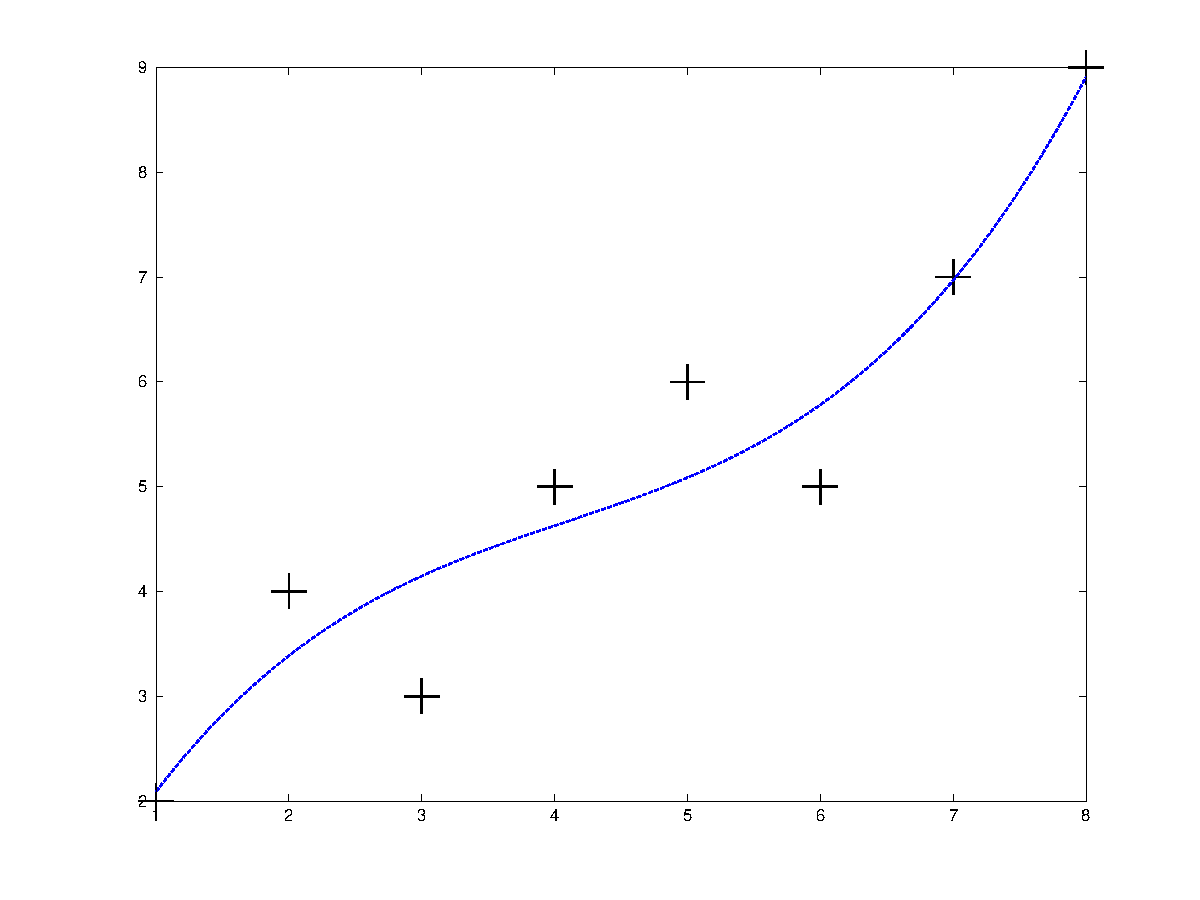
\includegraphics[width=8cm, keepaspectratio]{fig/polyfit.pdf}
  \end{figure}
\end{frame}

\subsection{Representación Gráfica}


\begin{frame}
\frametitle{Representación gráfica}
\begin{itemize}
\item Representar datos es sencillo e intuitivo
\item No hay que emocionarse con la representación gráfica
\item Sólo veremos curvas en el plano
\item ¿Necesitamos más?
\end{itemize}
\end{frame}

\defverbatim[colored]\testcode{
\begin{lstlisting}
>> x=linspace(0,500,100000);
>> plot(x,exp(-x/100).*sin(x))
\end{lstlisting}
}

\begin{frame}
\frametitle{Plot}
Representa curvas en el plano. $e^{-x/100}\sin x$ para $x\in[0,500]$
\testcode
\end{frame}

\begin{frame}
\frametitle{El resultado}
  \begin{figure}[h]
    \centering{}
    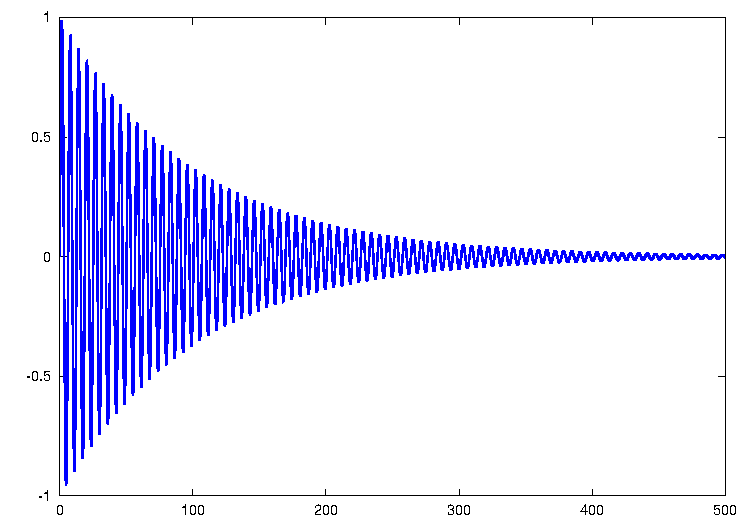
\includegraphics[width=8cm, keepaspectratio]{fig/abanico.pdf}
  \end{figure}
\end{frame}

\defverbatim[colored]\testcode{
\begin{lstlisting}
>> title('Una funcion cualquiera')
>> xlabel('Tiempo')
>> ylabel('Amplitud')
\end{lstlisting}
}

\begin{frame}
\frametitle{Etiquetas}
\testcode
\end{frame}

\begin{frame}
\frametitle{El resultado}
  \begin{figure}[h]
    \centering{}
    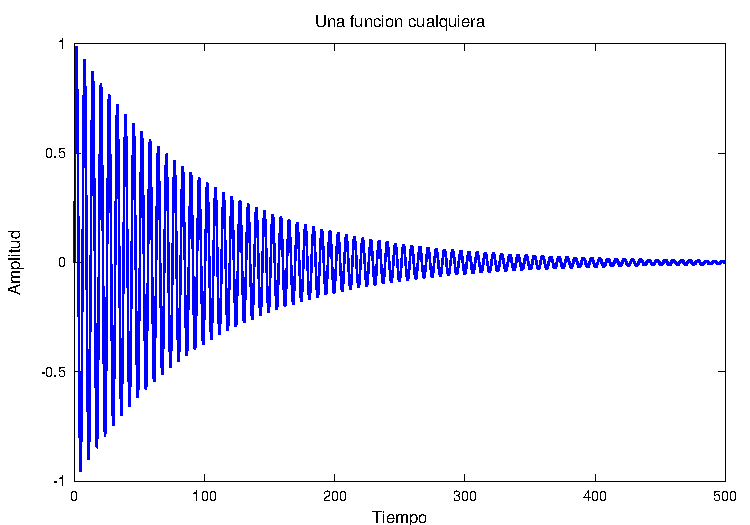
\includegraphics[width=8cm, keepaspectratio]{fig/abanico2.pdf}
  \end{figure}
\end{frame}

\defverbatim[colored]\testcode{
\begin{lstlisting}
>> x=linspace(-pi,pi,100);
>> plot(x,sin(x),'m:',...
x,cos(x),'k^',x,tan(x),'bx')
>> axis([-pi,pi,-2,2])
>> grid on
>> legend('linea de puntos magenta',...
          'triangulos negros',...
          'cruces azules') 
\end{lstlisting}
}
\begin{frame}
\frametitle{Estilos}
\testcode
\end{frame}

\begin{frame}
\frametitle{El resultado}
  \begin{figure}[h]
    \centering{}
    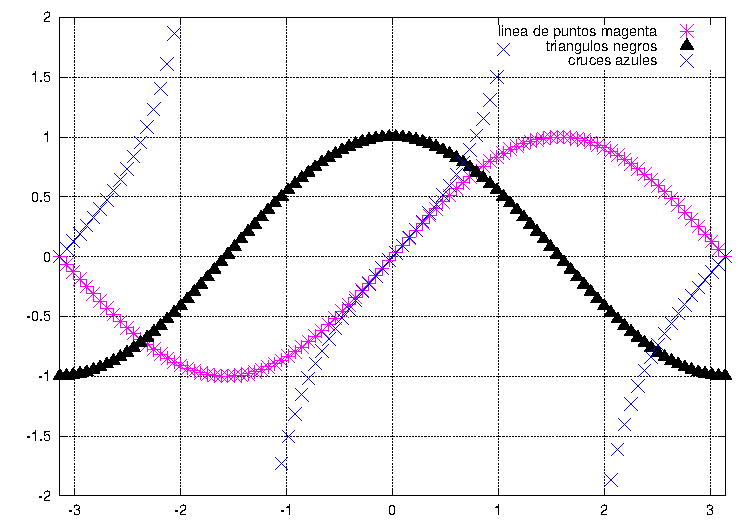
\includegraphics[width=8cm, keepaspectratio]{fig/trigplot.pdf}
  \end{figure}
\end{frame}

\begin{frame}
\frametitle{hold}
\begin{itemize}
\item La ventana gráfica se borra automáticamente cada vez que
  dibujamos algo
\item Para cambiar el comportamiento anterior se usa la función
  \emph{hold}
  \begin{itemize}
    \item \texttt{hold on} mantiene todo lo dibujado en la pantalla
    \item \texttt{hold off} vuelve al comportamiento inicial
  \end{itemize}
  \item Para borrar la ventana gráfica usamos \texttt{clf}
\end{itemize}
\end{frame}

\begin{frame}
\frametitle{\texttt{figure}}
\begin{itemize}
\item Las ventanas gráficas se manipulan con la función
  \texttt{figure}
\item Cada ventana gráfica tiene asociada un número entero
  \begin{itemize}
    \item \texttt{figure} se llama con un número que corresponde al de
      la ventana
    \item Si utilizamos un número que no corresponde a ninguna ventana
      existente crearemos una nueva con este número asociado
    \item Si utilizamos un número existente activaremos la ventana
      correspondiente
  \end{itemize}
\end{itemize}
\end{frame}

\defverbatim[colored]\testcode{
\begin{lstlisting}
>> x= linspace(-pi,pi,100);
>> subplot(2,2,1)
>> plot(x,sin(x))
\end{lstlisting}
}
\begin{frame}
  \frametitle{subplot}
  Es el comando que permite poner varios ejes en una misma figura
\testcode
Primero de los cuatro sectores.
\end{frame}

\begin{frame}
\frametitle{El resultado}
  \begin{figure}[h]
    \centering{}
    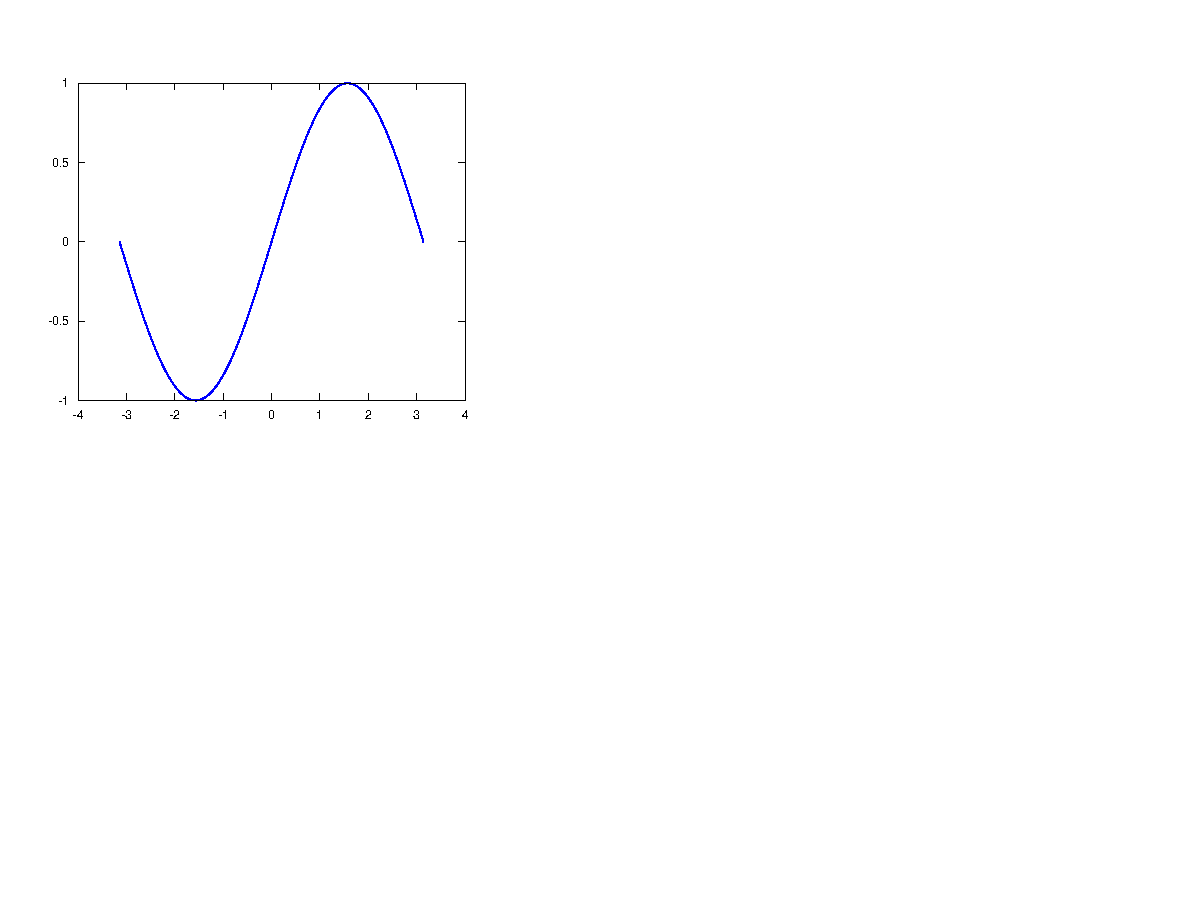
\includegraphics[width=8cm, keepaspectratio]{fig/subplot1.pdf}
  \end{figure}
\end{frame}


\defverbatim[colored]\testcode{
\begin{lstlisting}
>> subplot(2,2,2)
>> plot(x,cos(x))
>> subplot(2,2,3)
>> plot(x,sinh(x))
>> subplot(2,2,4)
>> plot(x,cosh(x))
\end{lstlisting}
}

\begin{frame}
\frametitle{subplot}
Ahora completamos los cuatro cuadrantes.
\testcode
\end{frame}

\begin{frame}
\frametitle{El resultado}
  \begin{figure}[h]
    \centering{}
    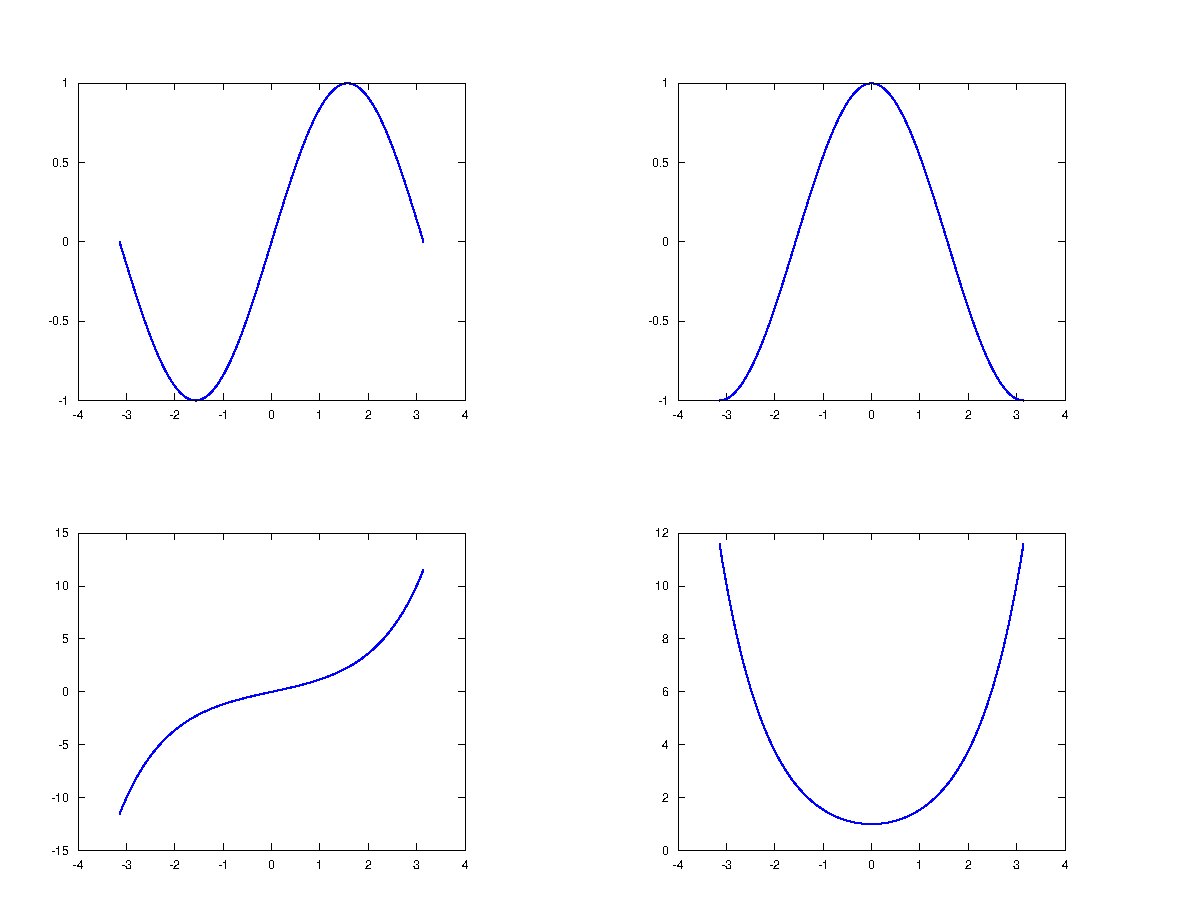
\includegraphics[width=8cm, keepaspectratio]{fig/subplot2.pdf}
  \end{figure}
\end{frame}

\begin{frame}
\frametitle{Otros comandos}
\begin{description}
\item[semilogx] Dibuja una curva con el eje x en escala logarítmica
\item[semilogy] Dibuja una curva con el eje y en escala logarítmica
\item[loglog] Dibuja una curva en escala logarítmica
\end{description}
\end{frame}

\begin{frame}
\frametitle{Ejercicio}

Representar en una misma ventana y dos frames (uno superior y otro
inferior) la función

\[ \sqrt{x} \sin(1/x)\ \ x \in[0.001,1]  \]

en escala normal y en escala semilogarítmica en el eje x.
\end{frame}

\begin{frame}
\frametitle{Comandos interesantes}
\begin{description}
\item[\texttt{get}, \texttt{set}] Cambia los atributos de un plot
  handle
\item[\texttt{text}] Pone texto en la figura
\item[\texttt{contour}] Isolíneas de una matriz de datos en 3D
\item[\texttt{griddata}] Interpola para el contour
\end{description}
\end{frame}


\end{document}
